\section{Reverse Engineering}\label{lit-reverseengineering}

\subsection{Introduction to Reverse Engineering}\label{lit-reverseengineering-introduction}

Reverse engineering is defined as ``to disassemble and examine or analyse in detail (a product or device) to discover the concepts involved in manufacture'' \citep{reverseengineeringdictionary}. According to \cite{chikofsky1990reverse} reverse engineering specifically of software involves the analysis of a system with the aim of:
\begin{itemize}
\item Identifying system components and relationships.
\item Generating a view of the system at a higher level of abstraction or in an alternative form.
\end{itemize}

System development can be seen as \textit{forward engineering}, moving from requirements and specification through design and implementation. \textit{Reverse engineering}, by definition the opposite, is a move from an implemented system back to designs \citep{roscoelooking}.

It can be sometimes claimed that software reverse engineering is a ``disreputable activity'', seeking to pull apart to use or copy others' solutions, potentially without permission. However it is also commonly used by the intellectual property owner as an aid to further development or maintenance \citep{roscoelooking}.

In an ideal world all systems would be developed in a clear and well documented manner, facilitating easy understanding of both structure and function. However developers are often faced with poorly documented and/or legacy systems which become extremely hard to comprehend by reading source code alone \citep{philippow2005approach,counsell2004design,meyer2006pattern}.

\cite{chikofsky1990reverse}, \cite{roscoelooking}, \cite{mamas2000towards}, and \cite{rasoolsurvey} all agree that reverse engineering can have the following significant legitimate benefits with regard to poorly documented or legacy systems:
\begin{itemize}
\item Maintenance - in order to make even small corrective changes to the system, let alone major changes, a good understanding of its overall function, structure and inter-component reliance is required.
\item Interoperability - allowing for the understanding of data flows and formats. This provides the ability to expand the system to interface with other systems for example through the transfer of data.
\item Security - reverse engineering can be a very effective tool in testing the level of security of a system, discovering unforeseen security holes and other potential problems or unexpected behaviour.
\item Behaviour Modification - an understanding of system operation is essential for modification or further expansion of the system.
\end{itemize}

Of these benefits aiding maintenance can be the most significant given that in cost terms maintenance is the most expensive stage of the software development lifecycle \citep{meyer2006pattern}.

In section \ref{lit-reverseengineering-goals} the goals and challenges of software reverse engineering are identified. Approaches to reverse engineering are covered in section \ref{lit-reverseengineering-approaches} before different types of language abstracted notations are detailed in section \ref{lit-reverseengineering-abstractnotation}. Available tools for software reverse engineering are detailed in section \ref{lit-reverseengineering-tools}, before being compared with regard to features provided.

\subsection{Goals of Software Reverse Engineering}\label{lit-reverseengineering-goals}

The overarching purpose of software reverse engineering is to aid clarity and promote understanding of a system in order to facilitate maintenance and further development \citep{chikofsky1990reverse}. Specifically the goal is therefore to identify components along with their relationships to facilitate the creation of understandable design-level representations of the system \citep{roscoelooking,chikofsky1990reverse}.

\cite{chikofsky1990reverse} defines three levels in which these representations can be seen:
\begin{itemize}
\item Requirements - the overall specification of the goals of the system, the problem it solves
\item Design - the specification of the overall system to meet the goal(s)/solve the problem(s) identified in requirements
\item Implementation - the actual code-level functionality
\end{itemize}

Reverse engineering techniques may yield a wide variety of information such as the quantification of algorithms, identification of design patterns used or illustration of general component interactions \citep{roscoelooking}. However it remains the overall goal to produce design-level information in a level of detail and abstraction suitable for developers who are non-expert in a system to gain as complete an understanding as they require \citep{chikofsky1990reverse,philippow2005approach}. For example UML recovery (recreation of UML diagrams illustrating system design and operation) is a frequent aim in reverse engineering \citep{roscoelooking}.

\subsubsection{Challenges}\label{lit-reverseengineering-challenges}

There are a number of challenges with regard to reverse engineering from source code, often owing to the inconsistent style and quality of code \citep{counsell2004design,uchiyama2011design,meyer2006pattern}, and success (the recreation of holistic systems designs) may vary widely depending on the methods used, the complexity, size and quality of the codebase \citep{counsell2004design}.

Commonly major programming languages (such as C++ and Java) have no support for in-built semantic definitions of structures such as design patterns. This leaves developers only the option of using code-level comments in natural language (possibly aided by comments in a set format compatible with javadoc for example), something which is highly variable depending on the developers and may be entirely inconsistent between different teams \citep{philippow2005approach}.

Software systems often contain poor design and component relationships further complicating analysis and comprehension of the code, with responsibilities being distributed throughout the system rather than compartmentalised \citep{meyer2006pattern}.

Even more formalised development approaches such as design patterns (section \ref{lit-reverseengineering-designpatterns}), by very definition a standardised way of implementing a solution, may have many different forms of concrete implementation or naming conventions \citep{uchiyama2011design}.

\clearpage
\subsection{Approaches to Software Reverse Engineering}\label{lit-reverseengineering-approaches}

To analyse system design a tool must analyse source code and extract relevant information. Commonly information is extracted from source code in a language-independent form (the main language abstracted notations are detailed in section \ref{lit-reverseengineering-abstractnotation}) building a representation of the code for analysis \citep{arcelli2005comparison}.

\subsubsection{Static and Dynamic Analysis}\label{lit-reverseengineering-staticdynamic}

The majority of approaches use ``static analysis'' where the source code is directly analysed \citep{shi2006reverse,arcelli2005comparison,flores2005reverse}. This can provide information into the structure and relationship of artefacts within the codebase and a complimentary ``dynamic analysis'' can be used where data is gathered at runtime, allowing the analysis of code behaviour during execution \citep{cerulo2006use,rasoolsurvey}

\subsubsection{Types of Analysis Process}\label{lit-reverseengineering-types}

\cite{rasoolsurvey} identify four main types of reverse engineering analysis:

\begin{itemize}
\item Structural - analysis of the structural relationships between different artefacts within the source code.
\item Behavioural - uses dynamic analysis of runtime data combined with static analysis to identify behavioural characteristics within the system.
\item Semantic - used in addition to structural and behavioural analysis to further refine understanding based upon information such as naming conventions. Primarily this aims to provide differentiation (for example of design patterns where the structure and/or behaviour are very similar - section \ref{lit-reverseengineering-designpatterns}).
\item Formal specification - used where available and a formal specification/approach was used during development, in effect a form of semantic analysis based upon more formalised criteria.
\end{itemize}

\subsubsection{Design Pattern Recognition}\label{lit-reverseengineering-designpatterns}

Design patterns, as initially identified and defined by \cite{gamma1995design}, are solutions to commonly occurring problems experienced in development. As they are frequently used, often core, constructs within software systems identification of design patterns from source code is often a goal of reverse engineering \citep{rasoolsurvey,shi2006reverse,arcelli2005comparison,uchiyama2011design}. Understanding of the design patterns used within a system can provide a significant step toward the overall goal of gaining a representation of the holistic function of the system \citep{counsell2004design}.

Identification of design patterns in existing code (``design pattern recovery'') is commonly attempted by transferring code into an abstract notation (as with most reverse engineering - section \ref{lit-reverseengineering-introduction}) before using pattern matching to identify specific uses of design patterns \citep{shi2006reverse,rasoolsurvey}. These processes can be iterative and themselves use design patterns for example SPQR uses a \textit{Pipes \& Filters} pattern to iteratively filter the source code into abstract notation until it reaches a suitable state for pattern recognition \citep{flores2005reverse}.

Identification of design patterns from source-code is non-trivial for a number of reasons. They are designed to support forward engineering without pattern classification or identification for reverse engineering \citep{shi2006reverse}. Many of the patterns are structurally (and often behaviourally) very similar \citep{rasoolsurvey} and can vary in concrete implementation.

Even a relatively simple pattern such as the Singleton \citep{gamma1995design} which is also one of the most widely used \citep{uchiyama2011design} can vary significantly in implementation as the following Java listing illustrates:

\begin{lstlisting}
public class SingletonA
{
    private static SingletonA instance = null;
    protected SingletonA() { }
    public static SingletonA getInstance()
    {
        if (SingletonA.instance == null)
            SingletonA.instance = new SingletonA();
        return SingletonA.instance;
    }
}

public class SingletonB 
{
    private static boolean hasInstance = false;
    public SingletonB() throws Exception
    {
        if (SingletonB.hasInstance)
            throw new Exception
                ("Can only have one instance");
        else
            SingletonB.hasInstance = true;
    }    
}

// create A
SingletonA a = SingletonA.getInstance(); 
// return same instance
SingletonA a2 = SingletonA.getInstance(); 
// create B
SingletonB b = new SingletonB();
// create B again (throw exception as already exists)
SingletonB b2 = new SingletonB();
\end{lstlisting}
\textit{Listing showing two alternative implementations of the Singleton in Java, adapted from \cite{gamma1995design} and \cite{uchiyama2011design}}

\subsection{Language Abstracted Notations}\label{lit-reverseengineering-abstractnotation}

Language abstracted notations such as those detailed in this section are useful in reverse engineering to represent programmatic function in a manner which is independent of the original (concrete) code syntax. Code layout becomes irrelevant so control-flow and data-flow can be more easily determined (\cite{fischer2007abstract};section \ref{lit-reverseengineering-introduction}).

\subsubsection{Abstract Syntax Tree (AST)}\label{lit-reverseengineering-ast}

Abstract Syntax Trees (ASTs) have been commonly used in code compilation as an intermediate data format between a source-code language and a machine/platform specific binary output, with programming language constructs represented as a tree \citep{fischer2007abstract,omgastm}. In this way ASTs capture the key structure of code in tree form without unnecessary syntactic details; ASTs are a pure representation of function without detail contained in concrete trees such as language-specific flow controls \citep{jones2003abstract}. ASTs are ``a formal representation of the syntactical structure of the software that is more amenable to formal analysis techniques than is the concrete or surface syntax of software'' \citep{omgastm}.

ASTs are constructed most commonly through source-code parsing but may also be built from generation or derivation processes from another form \citep{omgastm}.

An AST is a finite tree comprised of labelled and directed nodes with internal nodes representing operators and leaf nodes operands of the operators. Data structures that make up ASTs provide for a full collection of base compositional elements that are used by the source-code language \citep{omgastm}.

While there are different specific implementations of AST syntax they all have the same design basis and ethos, representing a hierarchical tree of control starting from the top and executing left-to-right with nodes indicating individual operations such as assignment and comparison \citep{fischer2007abstract}. An example of an AST can be seen in figure \ref{fig-lit-reverseengineering-astexample}.

\begin{figure}[hbtp]
\centering
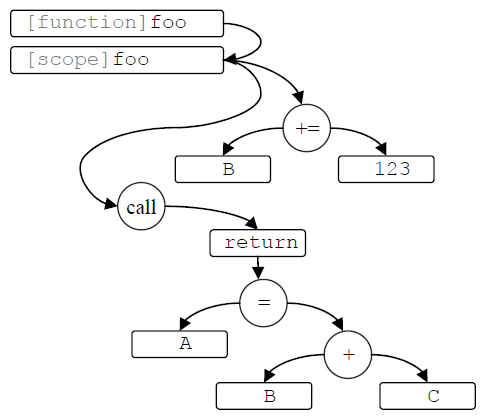
\includegraphics[scale=0.8]{sections/literature/reverseengineering/ast-example-misek}
\caption{AST Example \citep{misek2010mapping}}
\label{fig-lit-reverseengineering-astexample}
\end{figure}

The Object Management Group (OMG) have been attempting to derive a more formalised and widely accepted metamodel for ASTs, allowing for wider standardisation and use in the form of the AST MetaModel (ASTM) \citep{omgastm}.

\cite{omgastm} defines metamodels for three specific domains:
\begin{itemize}
\item Generic elements which are common in many languages represented by Generic Abstract Syntax Trees (GAST)
\item Language specific where individual languages purely are modelled by Language Specific Abstract Syntax Trees (SAST)
\item Propitiatory when elements of languages are modelled in inconsistent formats by Proprietary Abstract Syntax Trees (PAST)
\end{itemize}

\subsubsection{Abstract Semantic Graph (ASG)}\label{lit-reverseengineering-asg}

An Abstract Semantic Graph (ASG) is an AST containing extra information providing a richer picture. In addition to the nodes contained within an AST representing source-code entities, ASGs contain \textit{non-tree edges} showing relationships. These relationships connect references to declarations as well as declarations to types \citep{raghavan2004dex,mamas2000towards}. Figure \ref{fig-lit-reverseengineering-asgexample} shows a simple ASG including edge information from \cite{raghavan2004dex}.

\begin{figure}[hbtp]
\centering
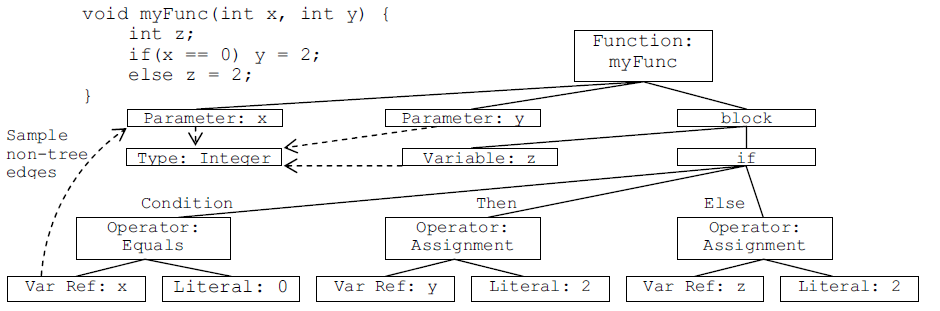
\includegraphics[scale=0.6]{sections/literature/reverseengineering/asg-example-raghavan}
\caption{ASG Example Showing \textit{non-tree edges} \citep{raghavan2004dex}}
\label{fig-lit-reverseengineering-asgexample}
\end{figure}

\subsubsection{XML Metadata Interchange (XMI)}\label{lit-reverseengineering-xmi}

XML Metadata Interchange (XMI) is part of the Object Management Group (OMG) Knowledge Discovery Metamodel (KDM). XMI is a XML schema (specific formal definition of XML structure) and XMI documents are XML-valid documents conforming to the schema \citep{omgxmi}.

It provides for model representation of Meta Object Facility (MOF) models in a standard XML format, commonly using the MOF definitions of Unified Modelling Language (UML - section \ref{lit-reverseengineering-uml}) both of which (MOF and UML) are also OMG standards \citep{omgmof,omgxmi}.

Provision is contained within the schema to further extend information types through the in-file definition of complex types, as well as the option to specify meta data including information about the XMI document itself (owner, descriptions, etc) \citep{omgxmi}. In addition to providing for abstract analysis of code parsed into XMI (the primary use of XMI within reverse engineering) there is also provision for generation of code from XMI and the interchange of XMI data, with the representative expressed functionality, between tools \citep{omgxmi}.

Although XMI can store data in different formats it is primarily used to encode UML data and supports different UML versions. Within the XMI schema every model class is described by an XML element that represents it \citep{omgxmi}. Below is a simple XMI example representing UML information of a class:

\begin{lstlisting}[language=XML]
<xmi:XMI xmlns:uml="http://www.omg.org/spec/UML/20110701"
xmlns:xmi="http://www.omg.org/spec/XMI/20110701">
<uml:Class name="C1" xmi:type=?uml:Class? xmi:id=?_1?>
<ownedAttribute xmi:type="uml:Property" xmi:id=?_2? name="a1"
visibility="private"/>
</uml:Class>
</xmi:XMI>
\end{lstlisting}
\textit{XMI XML listing of class C1 in UML format, from \cite{omgxmi}}

\subsubsection{Unified Modelling Language (UML)}\label{lit-reverseengineering-uml}

The Unified Modelling Language (UML) is an Object Management Group (OMG) specification for a visual language to document systems. It is designed to be applicable to all domains and platforms, enabling all software artefacts to be specified, constructed and documented. UML has the ability therefore to support round-trip engineering with source code being generated by and/or transformed into UML, this is a feature supported by a number of UML tools or UML-enabled environments \citep{omguml}.

\cite{omguml} identify the design principles of UML as follows:
\begin{itemize}
\item Modularity - grouping is used, applying the concept of strong cohesion and loose coupling
\item Layering - Package structures separate the language constructs from their use and an architectural pattern is used to separate concerns over different layers of abstraction
\item Extensibility - the language can be customised for specific platforms or domains either through the definition of new members or a new dialect
\item Reuse - through flexibility and granular construction the specification is suitable for wide reuse
\end{itemize}

UML can be used to represent numerous types of diagram, relationship and/or interaction within the system including class diagrams, use case diagrams and sequence diagrams. These diagrams can offer different levels of detail for example a class diagram can show just the class or include all members and properties contained within \citep{omguml}. Figures \ref{fig-lit-reverseengineering-umlexamplesimple} and \ref{fig-lit-reverseengineering-umlexampledetail} show simple UML class diagrams with an increasing level of detail contained within the same model.

\begin{figure}[hbtp]
\centering
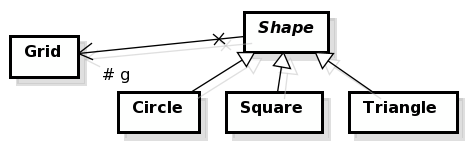
\includegraphics[scale=0.8]{sections/literature/reverseengineering/uml-class-simple-astah}
\caption{Simple UML Class Diagram showing inheritance and a relationships. Generated using reverse engineering in Astah Professional}
\label{fig-lit-reverseengineering-umlexamplesimple}
\end{figure}

\begin{figure}[hbtp]
\centering
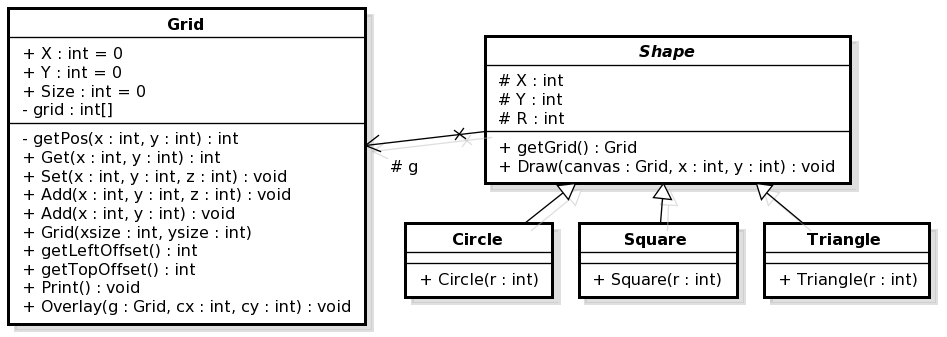
\includegraphics[scale=0.6]{sections/literature/reverseengineering/uml-class-detail-astah}\caption{UML Diagram of the relationships shown in figure \ref{fig-lit-reverseengineering-umlexamplesimple} but with added detail of properties and members}
\label{fig-lit-reverseengineering-umlexampledetail}
\end{figure}

\clearpage
\subsection{Tools for Software Reverse Engineering}\label{lit-reverseengineering-tools}

Generally tools for reverse engineering fall into two categories; those concerned with the identification of specific idioms such as design patterns (usually research projects) and those offering a fuller UML environment many with both forward and reverse engineering. In this section tools from both categories are identified and their features listed.

\subsubsection{Feature Comparison}\label{lit-reverseengineering-toolfeatures}

Table \ref{table-lit-reverseengineering-comptools} shows a comparison between reverse engineering tool features. Many of these tools are commercial and have no peer-reviewed information available in which case the data below is taken from the manufacturer's website. When tools with multiple possible versions offering different levels of features are covered the highest specification is used.
\clearpage
\begin{longtable}{| p{3cm} | p{2cm} | p{2cm} | p{3cm} | p{3cm} | p{3cm} |}

\hline

\textbf{Tool} & \textbf{Language\newline(s)} & \textbf{UML} & \textbf{Idioms} & \textbf{Notes}\\

\hline

FUJABA \citep{fujaba} & Java & UML forward and backward & Design Patterns, Idioms, Anti-patterns & MOF support for interoperability\\

\hline

DeMIMA \citep{demima} & Java & None & Design pattern recognition & None\\

\hline

PINOT \citep{pinot} & Java & None & Design pattern recognition & None\\

\hline

SPOOL \citep{spool} & Java (possible others such as C++ and Smalltalk) & None & Design pattern recognition & None\\

\hline

Osprey \citep{shi2006reverse} & Java, C++ and some support for C & None & Design pattern recognition & None\\

\hline

Columbus \citep{columbus} & C++ & None & Design pattern recognition & None\\

\hline

SPQR \citep{arcelli2005comparison} & Java & None & Design pattern recognition & None\\

\hline

DP++ \citep{philippow2005approach} & C++ & None & Design pattern recognition & Aimed at HPC applications\\

\hline

KT \citep{philippow2005approach} & Smalltalk & None & Design pattern recognition & None\\

\hline

Agile J Structure Views \citep{agilej} & Java & Class Diagrams & - & Eclipse plugin\\
\hline
Altova UModel \citep{umodel} & Java, C\#, VB.NET & UML 2.0 & - & Eclipse/Visual Studio plugin, XMI Support\\
%\hline
%\clearpage\\
%\hline
%\textbf{Tool} & \textbf{Language(s)} & \textbf{UML} & \textbf{Idioms} & \textbf{Notes}\\
\hline
ArgoUML \citep{argouml} & Java (with plugin options available for other languages) & Reverse engineering to class diagrams supported (plugin possibilities and creation tools for other UML diagrams) & - & -\\
\hline
Astah Professional \citep{astah} & Java, C++, C\# & UML 2.x & - & XMI Support\\
\hline
BOUML \citep{bouml} & C++, Java, PHP, MySQL & UML Projection & - & XMI Support\\
\hline
Enterprise Architect \citep{enterprisearchitect} & C++, Java, C\#, VB.Net, Visual Basic, Delphi, PHP, Python, ActionScript & All UML 2.3.1 Diagrams supported (unclear how many are supported in reverse engineering) & - & XMI Support\\
\hline
Rational Rhapsody (IBM) \citep{rationalrhapsody} & C++, C, Java, C\#, Ada & UML 2 & - & XMI Support\\
\hline
MagicDraw UML \citep{magicdraw} & Java, C++, C\#, CL (MSIL), COBRA IDL & UML 2 & - & XMI Support\\
\hline
Modelio \citep{modelio} & Java, C++, C\#, SQL & UML 2 & - & -\\
\hline
objectiF \citep{objectif} & C\#, C++, Java, VB.NET, BPEL, XSD, WSDL & UML 2 & - & Eclipse and Visual Studio plugin\\
\hline
Software Ideas Modeller \citep{softwareideasmodeller} & C\#, VB.NET, Java, .NET Assemblies & UML 2.4 & - & XMI Support\\
\hline
StarUML \citep{staruml} & Java & UML Class Diagrams & - & No longer maintained\\
\hline
Umbrello UML Modeller \citep{umbrello} & C++ & No automated creation but classes and relationships available for manual use in UML & - & -\\
\hline
Visual Paradigm for UML \citep{visualparadigm} & Java, C++ & UML 2 & - & XMI Support\\
\hline
Rational Rose (IBM) & Java, C++, Ada, VB & UML 2 & - & XMI Support\\
\hline
Borland Together & Java, C++, COBRA IDL & UML 1.4+2.0 & Design Pattern support in creation only & XMI Support\\
\hline
\caption{Comparison of Reverse Engineering Tools}
\label{table-lit-reverseengineering-comptools}
\end{longtable}
